\documentclass[11pt,a4paper,oneside]{article}
\usepackage[UTF8,adobefonts]{ctex}

\usepackage{wrapfig}
\usepackage{indentfirst}
\usepackage{amsmath}
\usepackage{float}
\usepackage{ulem}

\usepackage[top=1in,bottom=1in,left=1.25in,right=1.25in]{geometry}

\usepackage{color}
\usepackage{xcolor}

\usepackage{multirow}

\begin{document}

\begin{figure}[H]
 \centering
  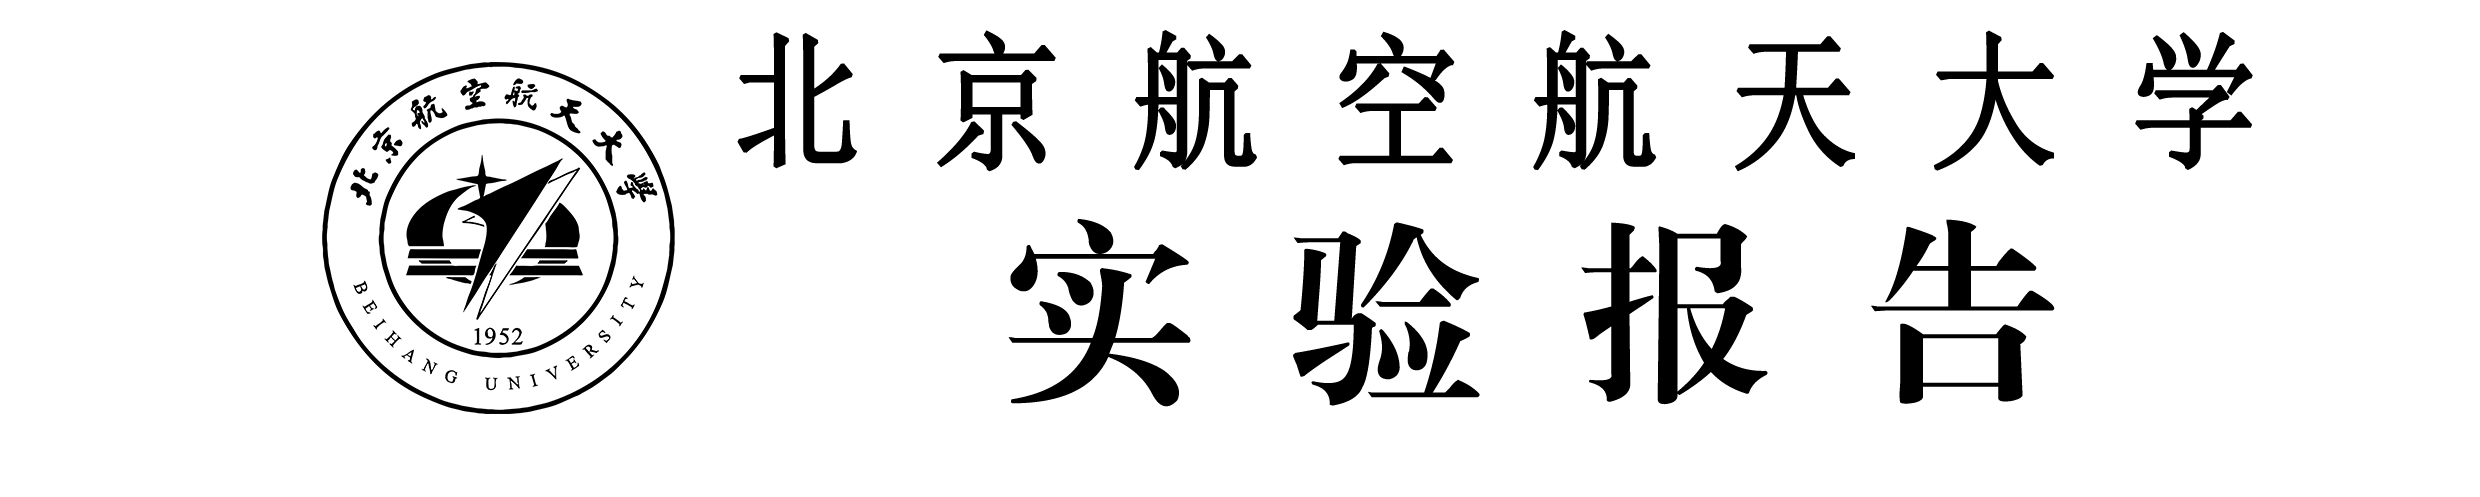
\includegraphics[width=13cm]{Image/表头.png}
\end{figure}
\begin{center}
\textbf{{\large 实验名称:\uline{          拉伸法测量钢丝弹性模量       }}}
\end{center}


\section*{一、实验目的}
\begin{enumerate}
\item 熟悉扭摆的构造及使用方法,掌握数字式计时器的准确适用;
\item 用扭摆测定几种不同形状物体的转动惯量,并与理论值进行比较;
\item 验证转动惯量平行轴定理;
\item 学习光杠杆法测弹性模量;
\item 熟练使用千分尺和游标卡尺,正确读取游标;
\end{enumerate}

\section*{二、实验原理}
\subsection*{实验1.拉伸法测钢丝弹性模量}
一条金属棒(丝),原长为L,截面积为A,在外力F作用下伸长$\delta L$。在弹性限度内,按照胡克定律有应力$(\sigma =\displaystyle\frac{F}{A})$与应变$(\varepsilon =\displaystyle\frac{\delta L}{L})$成正比,即$E=\displaystyle\frac{\sigma }{\varepsilon }$,E称为该金属的弹性模量,只取决于棒的材料性质。若金属棒为圆柱体,直径为D,则
\begin{center}
$ E=\displaystyle\frac{\sigma }{\varepsilon }=\displaystyle\frac{F/A}{\delta L/L}=\displaystyle\frac{4FL}{\pi D^{2}\delta L}$
\end{center}
其中F、L、D可以用一般的方法测得。而$\delta L$需要用光杠杆法测量。

\begin{figure}[H]
\centering
  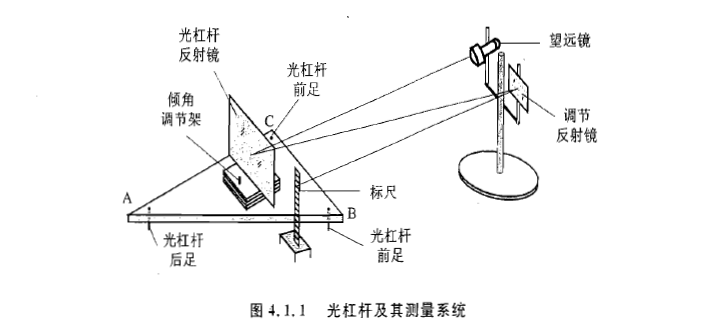
\includegraphics[width=12cm]{Image/光杠杆及其测量系统.png}
\end{figure}
光杠杆的结构如图4.1.1所示。
开始时光杠杆反射镜与标尺在同一平面,在望远镜上读到的标尺读数为$r_0$,当光杠杆反射镜的后足尖下降$\delta L$时,产生一个微小的偏角$\theta $,在望远镜上读到的标尺读数为$r_{i}$,则放大后的钢丝伸长量$C_{i}=r_i-r_0$。由图4.1.2可知
$$ \delta L_i=b\cdot \tan \theta \approx b\theta $$
式中,b为光杠杆前后足间的垂直距离,称光杠杆常数。
\begin{figure}[H]
\centering
  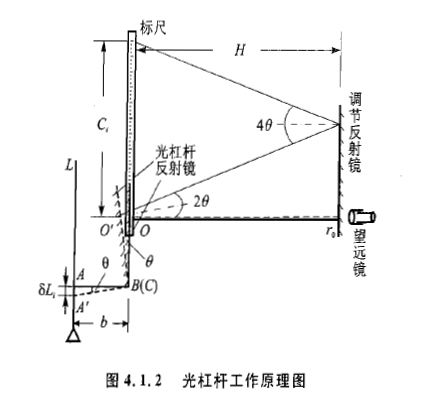
\includegraphics[width=7cm]{Image/光杠杆工作原理图.png}
\end{figure}
由于经光杠杆反射而进入望远镜的光线方向不变,故当平面镜旋转一定角度$\theta$之后,入射到光杠杆的光线方向就要偏转$4\theta$,因$\theta$甚小,OO'也甚小,故可认为平面镜到标尺的距离$H\approx O'r_0$,并有
\begin{center}
$2\theta \approx \tan 2\theta = \displaystyle\frac{C_i/2}{H},\theta =\displaystyle\frac{C_i}{4H}$
\end{center}
因此有
\begin{center}
$\delta L_i=\displaystyle\frac{bC_i}{4H}=WC_i,W=\displaystyle\frac{b}{4H}$
\end{center}
代入可得:

$$ E=\displaystyle\frac{16FLH}{\pi D^2bC_i}$$

\subsection*{实验2.扭摆法测转动惯量}
扭摆在其垂直轴l上装有一根薄片状的螺旋弹簧,用以产生恢复力矩。在轴的上方可以装上各种待测物体。将物体在水平面内转过一角度$\theta$后,在弹簧的恢复力矩作用下,物体就开始绕垂直轴作往返扭转运动。根据胡克定律,弹簧受扭转而产生的恢复力矩M与所转过的角度$\theta$成正比,即
\begin{center}
$M=-K\theta$
\end{center}
式中,K为弹簧的扭转常数。根据转动定律$M_{\text{总}}=I{\beta}$(I为物体绕转轴的转动惯量,$\beta$为角加速度),忽略轴承的摩擦阻力矩,则有$M_{\text{总}}=M$。由$\beta = \ddot{\theta}$,并令$\omega ^2=\displaystyle\frac{K}{I}$,得
\begin{center}
$\beta =\displaystyle\frac{d^2\theta}{dt^2}=-\displaystyle\frac{K}{I}\theta=-\omega ^2\theta $
\end{center}
上述方程表示扭摆运动具有角谐振动的特性:角加速度与角位移成正比,且方向相反。此方程的解为
\begin{center}
$\theta =A\cos (\omega t+\varphi )$
\end{center}
式中,A为谐振动的角振幅,$\varphi$为初相位角,$\omega$为角(圆)频率。此谐振动的周期为
\begin{center}
$ T=\displaystyle\frac{2\pi }{\omega}=2\pi \sqrt{\displaystyle\frac{I}{K}}$
\end{center}
利用上式,测得扭摆的摆动周期后,在I和K中任何一个量已知时即可计算出另一个量。

本实验用一个几何形状规则的物体(圆柱),其转动惯量($I_1$)可以根据它的质量和几何尺寸用理论公式直接计算得到,再算出本仪器弹簧的$K$值。若要测定其他形状物体的转动惯量,只需将待测物体安放在本仪器顶部的各种夹具上,测定其摆动周期,由上式即可换算出该物体绕转动轴的转动惯量。理论分析证明,若质量为$m$的物体绕过质心轴的转动惯量为$I_c$,当转轴平行移动距离x时,则此物体对新轴线的转动惯量变为$I_c+mx^2$。这称为转动惯量的平行轴定理。




\section*{三、实验仪器}
细钢丝、光杠杆、望远镜、标尺、拉力测量装置、钢卷尺、游标卡尺、螺旋测微器、扭摆、塑料圆柱体、金属空心圆筒、实心塑料(或木)球、金属细长杆(两个滑块可在上面自由移动)、数字式计时器、电子天平;三线摆、钢卷尺、电子秒表、圆环、气泡水平仪。

\section*{四、实验步骤}
\subsection*{实验1.拉伸法测钢丝弹性模量}
\subsubsection*{(1)调整测量系统}
\begin{enumerate}
\item 目测粗调
\item 调焦找尺
\item 细调光路水平
\end{enumerate}
\subsubsection*{(2)测量数据}
\begin{enumerate}
\item 首先预加10kg拉力,将钢丝拉直,然后逐次改变钢丝拉力,测量望远镜水平叉丝对应的标尺读数。
\item 根据量程及相对不确定度大小,选择合适的长度测量仪器,分别用卷尺、游标卡尺或千分尺测L、H、b各一次,测钢丝直径D若干次。
\end{enumerate}
\subsubsection*{(3)数据处理}
选择用逐差法、一元线性回归法或图解法计算弹性模量并估算不确定度。
\begin{enumerate}
\item L的误差限为0.3cm
\item H的误差限为0.5cm
\item b的误差限为0.02cm
\end{enumerate}

\subsection*{实验2.扭摆法测转动惯量}
\subsubsection*{(1)调整测量系统}
用水准仪调整仪器水平,设置计时器。
\subsubsection*{(2)测量数据}
\begin{enumerate}
\item 装上金属载物盘,测定其摆动周期$T_0$;将塑料圆柱体垂直放在载物盘上,测出摆动周期$T_1$,测定扭摆的弹簧扭转常数K。
\item 测定金属圆筒、塑料(或木)球与金属细长杆的转动惯量。列表时注意给出各待测物体转动惯量的测量公式(金属圆筒$I_2$、塑料球$I_3$以及金属细长杆$I_4$)和理论计算公式(金属圆筒$J_2$、塑料球$J_3$ 以及金属细长杆$J_4$)。
\item 验证转动惯量平行轴定理。将滑块对称地放置在细杆两边的凹槽内(此时滑块质心离转轴的距离分别为5.00、10.00、15.00、20.00、25.00(单位:cm))测出摆动周期$T_5i$。若时间许可,还可以将两个滑块不对称放置(例如分别取5.00与10.00,10.00与15.00,
15.00与20.00,20.00与25.00(单位:cm)),这样采用图解法验证此定理时效果更好。
\item 测量其他常数。利用电子天平,测出塑料圆柱、金属圆筒、塑料(或木)球与金属细长杆的质量,并记录有关物体的内、外径和长度。
\end{enumerate}
\subsubsection*{(3)数据处理}
\begin{enumerate}
\item 设计原始数据记录表格;
\item 算出金属圆筒、塑料(或木)球和金属细长杆的转动惯量$I_2$、$I_3$、$I_4$,并与理论计算值$J_2$、$J_3$、$J_4$比较,求百分差;
\item 验证平行轴定理。
\end{enumerate}
\section{五、数据处理}
\subsection{1.拉伸法侧钢丝弹性模量}
\subsubsection{(1)原始数据}
1. 钢丝长$L = [L]cm$,平面镜到标尺$H = [H]cm$,光杠杆前后足$b = [b]cm$。

2. 直径D
\begin{tabular}{|c|c|c|c|c|c|c|}
\hline 
D & 1 & 2 & 3 & 4 & 5 & 平均 \\ 
\hline 
(mm) & • & • & • & • & • & • \\ 
\hline 
\end{tabular} 

3. 读数
\begin{tabular}{|c|c|c|c|c|c|c|c|c|c|}
\hline 
加力(kg) & 10.000 & 12.000 & 14.000 & 16.000 & 18.000 & 20.000 & 22.000 & 24.000 & 26.000 \\ 
\hline 
加力读数 & • & • & • & • & • & • & • & • & • \\ 
\hline 
减力读数 & • & • & • & • & • & • & • & • & • \\ 
\hline 
平均 & • & • & • & • & • & • & • & • & • \\ 
\hline 
\end{tabular} 

\subsubsection{(2)数据处理}
1. 用逐差法计算弹性模量

令$k = 2n-1$,则$n = 5$,故$C_i = r_{i+5}-r_i(i = 1,2,3,4)$。
\begin{tabular}{|c|c|c|c|c|c|}
\hline 
组数(i) & 1 & 2 & 3 & 4 & 平均 \\ 
\hline 
$r_{i+5}-r_i$ & • & • & • & • & [平均] \\ 
\hline 
\end{tabular} 
又$E= \displaystyle\frac{16FLH}{\pi D^2bC_i}$,$F = \Delta mg$,$\Delta m = m_{i+5}-m{i}=10.000kg$,$C_i = [平均]cm$:

$\therefore E = \displaystyle\frac{16\Delta mgLH}{\pi D^2bC_i} = [E]$

2. 计算不确定度
对于L、H、b,只测量一次,不确定度只有B类分量

$\Delta L = 0.3cm$,$\Delta H = 0.5cm$,$\Delta b = 0.02cm$。

$u(L) = \displaystyle\frac {\Delta L}{\sqrt {3}} = 0.173cm$

$u(H) = \displaystyle\frac {\Delta H}{\sqrt {3}} = 0.289cm$

$u(b) = \displaystyle\frac {\Delta b}{\sqrt {3}} = 0.0115cm$

对于D,测量次数$k= 5$,则:

$u_a(D) = \sqrt{\displaystyle\frac{\sum (x_i-\bar{x})^2}{k(k-1)}}= \sqrt{\displaystyle\frac{\bar{x^2} - \bar{x}^2}{k-1}} = [uaD]mm$

$u_b(D) = \displaystyle\frac{\Delta D}{\sqrt{3}} = 0.00289mm$

$\therefore u(D) = \sqrt{u_a^2(D)+u_b^2(D)} = [uD]mm$

对于C,有:

$u_a(C) = \sqrt{\displaystyle\frac{\bar{C^2}-\bar{C}^2}{4-1}}=[uaC]cm$

$u_b(C) = \displaystyle\frac{\Delta 仪}{\sqrt{3}} = 0.0289cm$

$\therefore u(C) = \sqrt{u_a^2(C)+u_b^2(C)} = [uC]mm$

由$\displaystyle\frac{u(E)}{E} = \sqrt{[\displaystyle\frac{u(L)}{L}]^2+[\displaystyle\frac{u(H)}{H}]^2+[\displaystyle\frac{2u(D)}{D}]^2+[\displaystyle\frac{u(C)}{C}]^2+[\displaystyle\frac{u(b)}{b}]^2} = [比值]$

$\therefore u(E) = [uE]Pa$

$E \pm u(E) = ([E]\pm [uE])Pa$

\subsection{2.扭摆法测转动惯量}
\subsubsection{(1)原始数据}
\begin{tabular}{|c|c|c|c|c|}
\hline 
• & 塑料圆柱 & 金属圆筒 & 球 & 细杆 \\ 
\hline 
质量/g & • & • & • & • \\ 
\hline 
尺寸/mm & • & • & • & • \\ 
\hline 
\end{tabular} 

\begin{tabular}{|c|c|c|c|c|c|c|}
\hline 
• & t1 & t2 & t3 & t4 & t5 & 平均 \\ 
\hline 
物盘 & • & • & • & • & • & • \\ 
\hline 
盘+圆柱 & • & • & • & • & • & • \\ 
\hline 
盘+圆筒 & • & • & • & • & • & • \\ 
\hline 
圆球 & • & • & • & • & • & • \\ 
\hline 
细长杆 & • & • & • & • & • & • \\ 
\hline 
\end{tabular} 

1. 计算扭转常数k

$I_柱 = \displaystyle\frac{1}{8}MD^2$

$M = [塑料圆柱质量]kg$

$D = [塑料圆柱直径]m$

代入得

$I_柱 = [I柱]kg \cdot m^2$

由$T = 2\pi \sqrt{\displaystyle\frac{I}{K}}$,得$k = \displaystyle\frac{4\pi ^2I_柱}{T_1^2-T_0^2}$,其中$T_1$为盘+柱的周期,$T_0$为盘的周期。

得$k = [k]kg\cdotm^2/s^2$

2. 金属圆筒的转动惯量

$计算值I_筒 = \displaystyle\frac{k}{4\pi }(T_2^2-T_0^2) = [计算I筒]kg\cdot m^2$

$理论值J_筒 = \displaystyle\frac{1}{8}M(D_内^2+D_外^2) = [理论J筒]kg\cdot m^2$

$相对误差 \eta =\displaystyle\frac{\left | I-J \right |}{I}\times 100\% = [相对误差2]$

3. 球的转动惯量

$计算值I_球 = \displaystyle\frac{k}{4\pi }T_3^2 = [计算I球]kg\cdot m^2$

$理论值J_球 = \displaystyle\frac{1}{10}MD^2 = [理论J球]kg\cdot m^2$

$相对误差 \eta =\displaystyle\frac{\left | I-J \right |}{J}\times 100\% = [相对误差3]$

4. 细杆的转动惯量

$计算值I_杆 = \displaystyle\frac{k}{4\pi }T_4^2 = [计算I杆]kg\cdot m^2$

$理论值J_杆 = \displaystyle\frac{1}{12}ML^2 = [理论J杆]kg\cdot m^2$

$相对误差 \eta =\displaystyle\frac{\left | I-J \right |}{J}\times 100\% = [相对误差4]$

5. 验证平行轴定理

滑块质量$m_1 = [m1]kg$,$m_2 = [m2]kg$
$d_外 = [d外]mm$,$d_内= [d内]mm$,$l = [l]mm$

\begin{tabular}{|c|c|c|c|c|c|c|}
\hline 
位置cm\次数 & 1 & 2 & 3 & 4 & 5 & 平均 \\ 
\hline 
5 & • & • & • & • & • & • \\ 
\hline 
10 & • & • & • & • & • & • \\ 
\hline 
15 & • & • & • & • & • & • \\ 
\hline 
20 & • & • & • & • & • & • \\ 
\hline 
25 & • & • & • & • & • & • \\ 
\hline 
\end{tabular} 

取$x = d^2$,$y = T^2$,设$y = bx+a$

由一元线性回归运算

$b= \displaystyle\frac{\bar{x}\bar{y}- \bar{xy}}{\bar{x}^2-\bar{x^2}}=[b]$

$a = \bar{y} - b\bar{x} = [a]$

$r = \displaystyle\frac{\bar{xy}- \bar{x}\bar{y}}{\sqrt{(\bar{x^2}-\bar{x}^2)(\bar{y^2}-\bar{y}^2)}} = [r]$

线性关系强烈

$\therefore T_i^2 = [b]d_i^2+[a]$

理论值$J_{滑1} = \displaystyle\frac{1}{16}m_1(D_内^2+D_外^2) + \displaystyle\frac{1}{12}m_1h^2 = [I滑1]kg\cdot m^2$

理论值$J_{滑2} = \displaystyle\frac{1}{16}m_2(D_内^2+D_外^2) + \displaystyle\frac{1}{12}m_2h^2 = [I滑2]kg\cdot m^2$

依据平行轴定理有$J_杆 + J_{滑1} +J_{滑2} + (m_1 + m_2)d^2 = I = \displaystyle\frac{k}{4\pi ^2}T_i^2$

整理得$T_i^2 = [系数1]d_i^2 + [系数2]$;

对比可验证平行轴定理。

\end{document}